\documentclass[12pt, a4paper]{article}

\usepackage[medium]{titlesec}
\usepackage{graphicx}
\usepackage{caption}
\usepackage{amsmath}
\usepackage{amsthm}
\usepackage[legalpaper, portrait, margin=1.2in]{geometry}
\usepackage{wrapfig}
\usepackage{varwidth}
\usepackage{listings}
\usepackage{amssymb}
\usepackage{enumitem}
\usepackage{bm}
\usepackage{enumitem}

\allowdisplaybreaks  % will allow page break in align environment

\begin{document}
	
	\setlength{\parindent}{0pt}
	\captionsetup{justification=centering}
	\lstset{
		showstringspaces=false
	}
	
	
	\begin{titlepage}
		\LARGE
		\textbf{7.5}
		\begin{center}
			\vspace*{7cm}
			
			\LARGE
			\textbf{Mathematical Methods}
			\\
			\vspace{1cm}
			\textbf{Pad\'e Approximants}
			
			\vspace{0.5cm}
		\end{center}
	\end{titlepage}

\section{Introduction}	
	
\subsubsection*{Programming Task: Writing Programs A and B}

The programs written for this task can be found on pages \pageref{Program_A} and \
\pageref{Program_B}. From the numpy package in Python, I use the \texttt{lstsq} function \
as an equivalent of \texttt{mldivide} from Matlab. I first tested Program A for basic \
functions such as f(x) = 0 with different values of L and M. Then I carried out testing \
with more complex functions such as f(x) = sin(x) and confirming the $O(x^{L+M+1})$ \
accuracy via polynomial division of the results.


\subsubsection*{Question 1}

Using the binomial expansion, we obtain,
\begin{flalign*}
	f_{1}(x) = 1 + \frac{x}{2} - \frac{x^{2}}{8} + \frac{x^{3}}{16} &&
\end{flalign*}
with the following formula for the coefficients,
\begin{flalign*}
	c_{0} = 1, \quad c_{1} = \frac{1}{2}, \quad c_{k} = \frac{ (-1)^{k-1}(2k-3)! }{ 2^{2k-2}k!(k-2)! } \text{ for } \ 
	k \geq 1. &&
\end{flalign*}

The radius of convergence can be found via the ratio test.
\begin{flalign*}
	\text{Radius} & = \lim_{k \to \infty} \left| \frac{ c_{k} }{ c_{k+1} } \right| &&\\
	& = \lim_{k \to \infty}\left| \frac{ (2k-1)(2k-2) }{ 4(k+1)(k-1) } \right| &&\\
	& = 1
\end{flalign*}
This means that the Pad\'e approximant will only be useful within the disk of radius 1 \ 
centred at 0 in the complex plane. Also, the further from 0 you go, the more terms of \ 
the power series are required for a precise result. Therefore, approximants with a \ 
lower value of L+M+1 become much less useful in these cases.
\\

Taking $x = 1$ in the power series, we obtain $\sum_{k = 0}^{\infty}c_{k}$. Since this converges, the \
sequence of partial sums $\sum_{k = 0}^{N}c_{k}$ converges. This convergence is illustrated in figure\ 
\ref{q1_fig1}.

\vspace{0.3cm}
\begin{minipage}{\textwidth}
	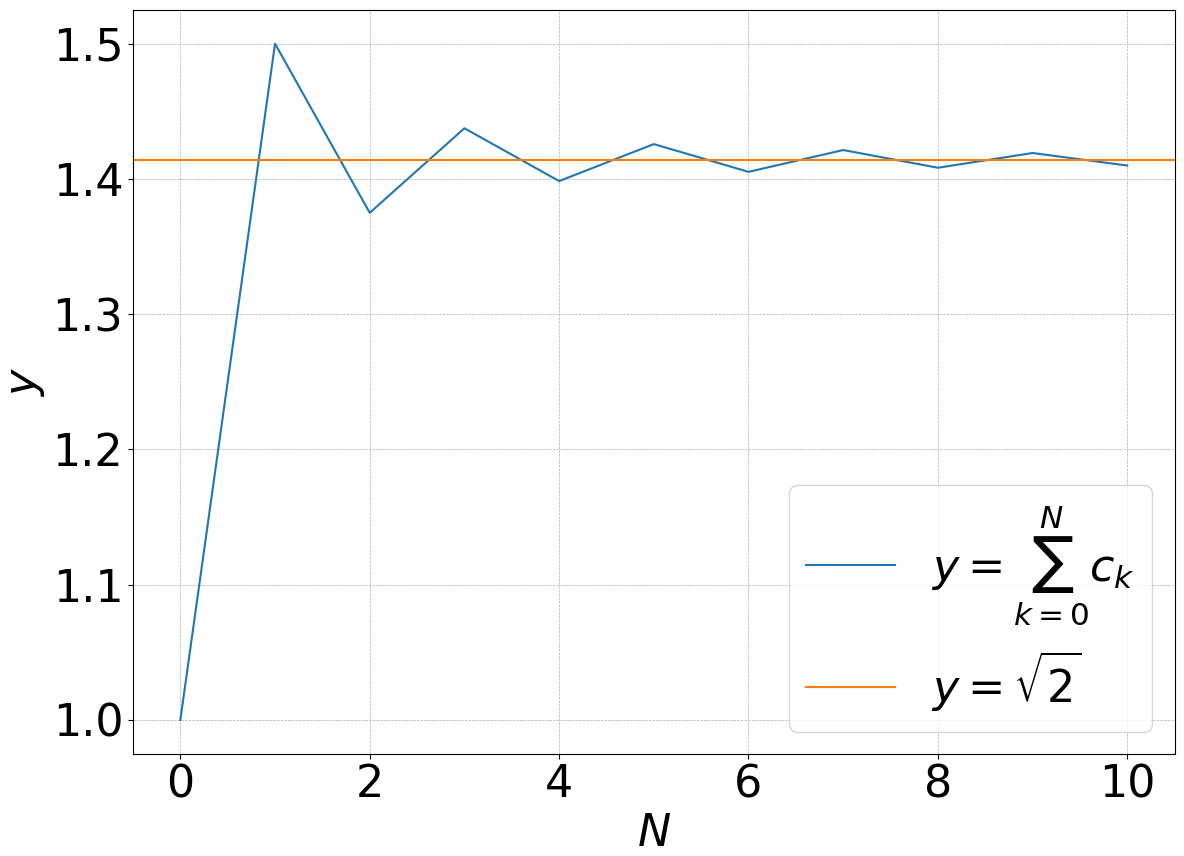
\includegraphics[width=\linewidth]{q1_fig1}
	\captionof{figure}{Line graph of partial sums}
	\label{q1_fig1}
\end{minipage}
\vspace{0.1cm}

We notice that the partial sums oscillate above and below $\sqrt{2}$, with the error getting smaller\
as $k$ increases. \\

We use the Lagrange form of the remainder for a Taylor expansion to estimate the error of the \
partial sum as an estimate of $\sqrt{2}$. The remainder at $x = 1$ will be,
\begin{flalign*}
	R_{N}(1) = \frac{ f_{1}^{(N+1)}(\xi) }{ (N+1)! } &&
\end{flalign*}
for some real number $\xi$ between 0 and 1 and following simplifications, we have,
\begin{flalign*}
	|R_{N}(1)|  = \frac{ (2N-1)! }{ 2^{2N}(N-1)!(N+1)! } (1+\xi)^{ -N + \frac{1}{2} } &&
\end{flalign*}
\\
Using the function \texttt{find\textunderscore xi} in the program on page \pageref{Question_1}, \ 
we find that $\xi$ is small and decreases as $N$ increases. For example, for $N = 3$, $\xi$ = 0.230; \ 
for $N = 10$, $\xi = 0.0681$ and for $N = 50$, $\xi = 0.0138$. Then the \
\texttt{print\textunderscore xi\textunderscore factor} also in the program on page \pageref{Question_1} \
can be used to show that for $N < 80$,  $ 0.5 \leq (1+\xi)^{ -N + \frac{1}{2} } \leq 0.7$. Hence, \
we have,
\begin{flalign}
	R_{N}(1)  &\leq 0.7 \cdot \frac{ (2N-1)! }{ 2^{2N}(N-1)!(N+1)! } && \nonumber \\
	&= 0.7 \cdot \frac{1 \cdot 3 \cdot 5 \cdot ... \cdot (2N - 1) }{ 2 \cdot 4 \cdot 6 \cdot ... \cdot 2N} \
	\cdot \frac{1}{2N+2} \label{error_eq}
\end{flalign}
We prove the following lemma:
\begin{flalign*}
	\frac{1 \cdot 3 \cdot 5 \cdot ... \cdot (2N - 1) }{ 2 \cdot 4 \cdot 6 \cdot ... \cdot 2N} \leq \ 
	\frac{1}{\sqrt{2N}}  && \\
	\text{Proof: } \left( \frac{1 \cdot 3 \cdot 5 \cdot ... \cdot (2N - 1) }{ 2 \cdot 4 \cdot 6 \cdot ... \cdot 2N}\ 
	\right)^{2} &= \frac{1 \cdot 1}{2 \cdot 2} \ 
	\cdot \frac{3 \cdot 3}{4 \cdot 4} ...\frac{(2N-1) \cdot (2N-1)}{2N \cdot 2N} && \\
	&= \frac{1 \cdot 3}{2 \cdot 2} \cdot \frac{3 \cdot 5}{4 \cdot 4} ... \ 
	\frac{(2N-1) }{(2N)^{2}} && \\
	&\leq \frac{2N-1}{(2N)^{2}} \text{ ~since~ } (n-1)(n+1) = n^{2}-1 \leq n^{2} && \\
	&\leq 1/2N ~~~~~~~~~~~~~~~~~~~~~~~~~~~~~~~~~~~~~~~~~~~~~~~~~~~ \qed
\end{flalign*}
Applying the lemma to (\ref{error_eq}), we obtain the following overestimate for the error as $N$ increases:
\begin{flalign}
	|R_{N}(1)|  \approx \frac{ 0.7 }{ (2N+2)\sqrt{2N} } \label{q1_eq2}
\end{flalign}
Figure \ref{q1_fig2} illustrates this as an error bound. We can see that this gives an accurate 
approximation of the error.

\vspace{0.3cm}
\begin{minipage}{\textwidth}
	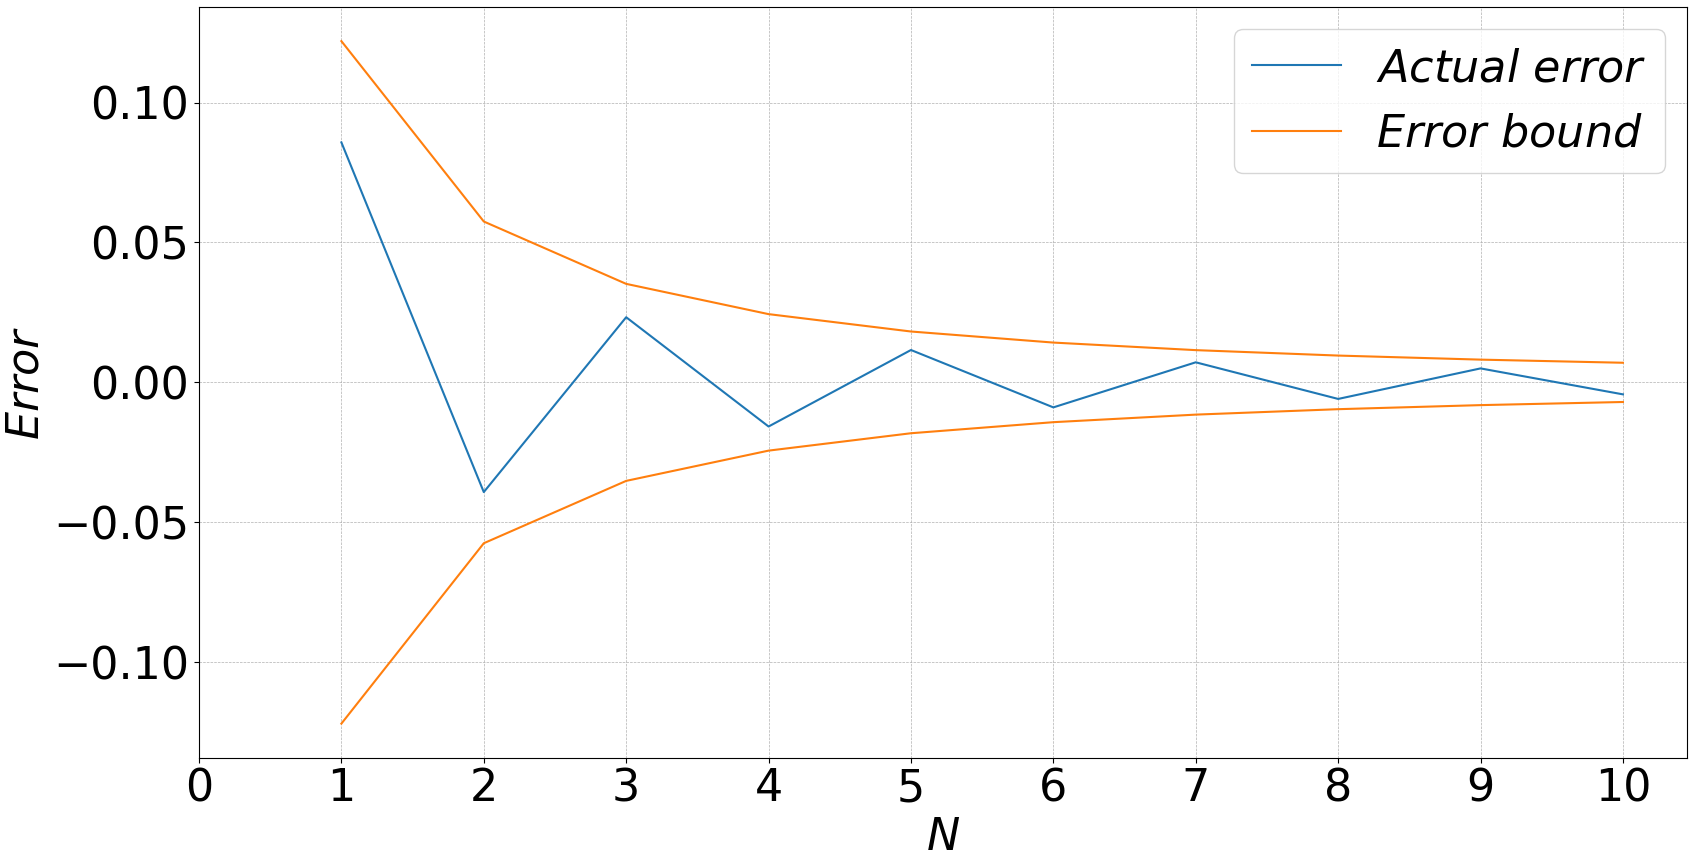
\includegraphics[width=\linewidth]{q1_fig2}
	\captionof{figure}{Actual error and estimated erro of the partial sum as an estimate of $\sqrt{2}$}
	\label{q1_fig2}
\end{minipage}
\vspace{0.1cm}

We know $(1+\xi)^{-N + \frac{1}{2}}$ is relatively unchanged when $N$ is increased by $1$. Thus taking \
the ratio of $R_{N}(1)$ and $R_{N+1}(1)$ shows that incrementing $N$ by $1$ decreases the error by \
very close to $\frac{ 2N+1 }{ 2N+4 }$. Hence the larger N is, the less the percentage decrease of error \
is for increasing N.


\subsubsection*{Question 2}

It is now much more difficult to obtain a theoretical result for the error, so we investigate $R_{L,L}(1)$\
as an estimate of $\sqrt{2}$ numercially. The results in the table below show the error of the approximant\
for different values of $L$.
\vspace{0.3cm}

\begin{minipage}{\textwidth}\centering
	\begin{tabular}{|l|l|}
	\hline
	\multicolumn{1}{|c|}{$L$} & \multicolumn{1}{c|}{Error}                  \\ \hline
	\multicolumn{1}{|c|}{0}   & \multicolumn{1}{c|}{0.41421356237309515}    \\ \hline
	\multicolumn{1}{|c|}{1}   & \multicolumn{1}{c|}{0.014213562373095234}   \\ \hline
	\multicolumn{1}{|c|}{2}   & \multicolumn{1}{c|}{0.00042045892481934466} \\ \hline
	\multicolumn{1}{|c|}{3}   & \multicolumn{1}{c|}{1.2378941142587863e-05} \\ \hline
	4                         & 3.644035522221145e-07                       \\ \hline
	5                         & 1.072704058913132e-08                       \\ \hline
	6                         & 3.1577518377901015e-10                      \\ \hline
	7                         & 9.29567534058151e-12                        \\ \hline
	8                         & 2.737809978725636e-13                       \\ \hline
	9                         & 7.993605777301127e-15                       \\ \hline
	10                        & 4.440892098500626e-16                       \\ \hline
	11                        & 2.220446049250313e-16                       \\ \hline
	12                        & 2.220446049250313e-16                       \\ \hline
	13                        & 6.661338147750939e-16                       \\ \hline
	14                        & 6.661338147750939e-16                       \\ \hline
	15                        & 2.220446049250313e-16                       \\ \hline
	\end{tabular}
\end{minipage}
\vspace{0.3cm}

\begin{minipage}{\textwidth}
	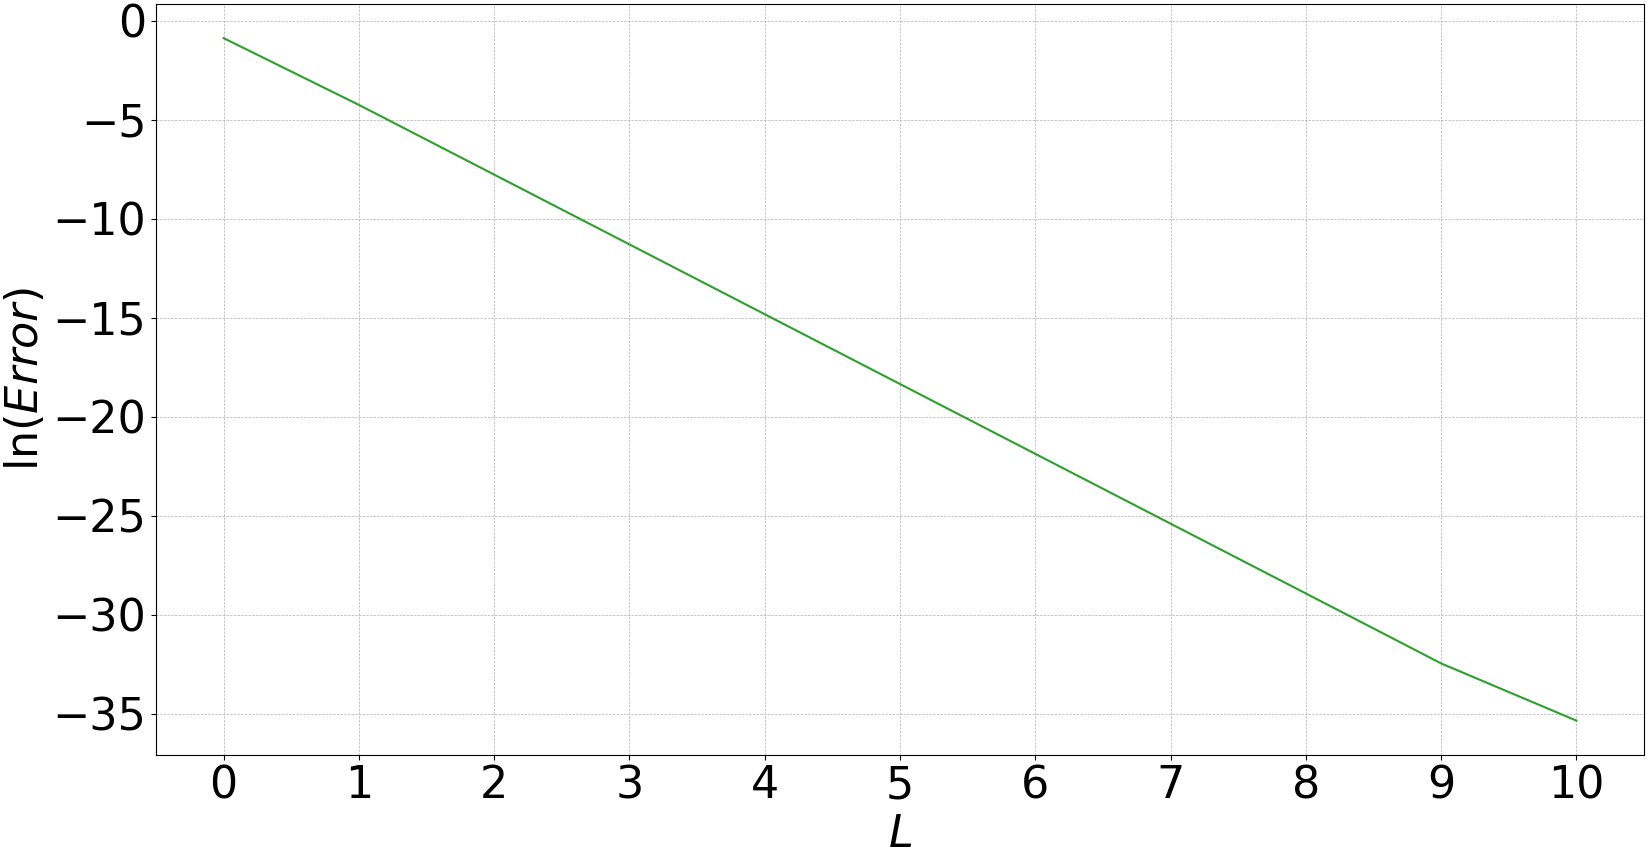
\includegraphics[width=\linewidth]{q2_fig1}
	\captionof{figure}{Plot of $L$ against $\ln(Error)$}
	\label{q2_fig1}
\end{minipage}
\vspace{0.3cm}

From figure \ref{q2_fig1}, we see that for $L \leq 10$, the error decreases exponentially.
We observe from the table that the minimum value of the error for $L \leq 15$ is 2.220446049250313e-16.\ 
This must be true in general since this is exactly the machine precision, i.e. it is the  difference between 1.0 and\ 
the smallest 64-bit double precision floating-point value larger than 1.0. Hence, the machine precision\ 
determines the smallest error.
\\

In cases where the matrix used to solve equation (4) is non-singular, iterative improvement will make no\ 
difference since the exact solution is found so no more improvements can be made. The determinant of the\
matrix in question approaches 0 as $L$ increases. The \texttt{lstsq} function which I have used as the\ 
Python equivalent of \texttt{mldivide} finds the least-squares solution of the equation $A\mathbf{x} = \mathbf{b}$. 
Suppose for some $L$ the determinant of the matrix used to solve equation (4) were 0 and let the least\ 
squares solution for the $q_{k}$ be $\mathbf{y}$. Then $\mathbf{b}-A\mathbf{y}$ will be orthogonal to \ 
$A\mathbf{x}$ for any $\mathbf{x}$. Hence no more improvements can be made in this case either.
\\

In addition, the limit on the error is cased my the machine precision, not the solution to equation (4).\ 
Thus iterative improvement would have no effect on the minimum error.
\\

In the power series of $R_{L,L}(x)$, the first $2L+1$ terms match that of $f_{1}(x)$. The error of\ 
$R_{L,L}(1)$ is much less than the power series estimate of $\sqrt{2}$ for the same number of matching terms.\
For instance, with $L = 5$, the error of the Pad\'e approximant is $1.07 \times 10^{-8}$ while for\ 
$N=10$ the error from the partial sum is $4.28 \times 10^{-2}$. This is surprising because using the same\
amount of information, a much more accurate estimate is obtained. This can be explained by the fact that\ 
as we approach the radius of convergence the error power series expansion of $f_{1}(x)$ diverges at a\
faster rate than the error term from the power series expansion of $R_{L,L}(x)$.
\\

It is then clear that the Pad\'e approximant should be used as an estimate of $\sqrt{2}$ to specified accuracy\
in all cases. The error estimation \ref{q1_eq2} shows that to have an error of $2.22\times10^{-16}$, which\ 
only requires $L=11$ for the Pad\'e approximant, you would need $N$ to be close to 100,000. Even if you wanted\ 
more accuracy than this, that wouldn't be possible with 64-bit floats since $2.22\times10^{16}$ is the\ 
machine precision.


\subsubsection*{Question 3}

\begin{minipage}{\textwidth}\centering
	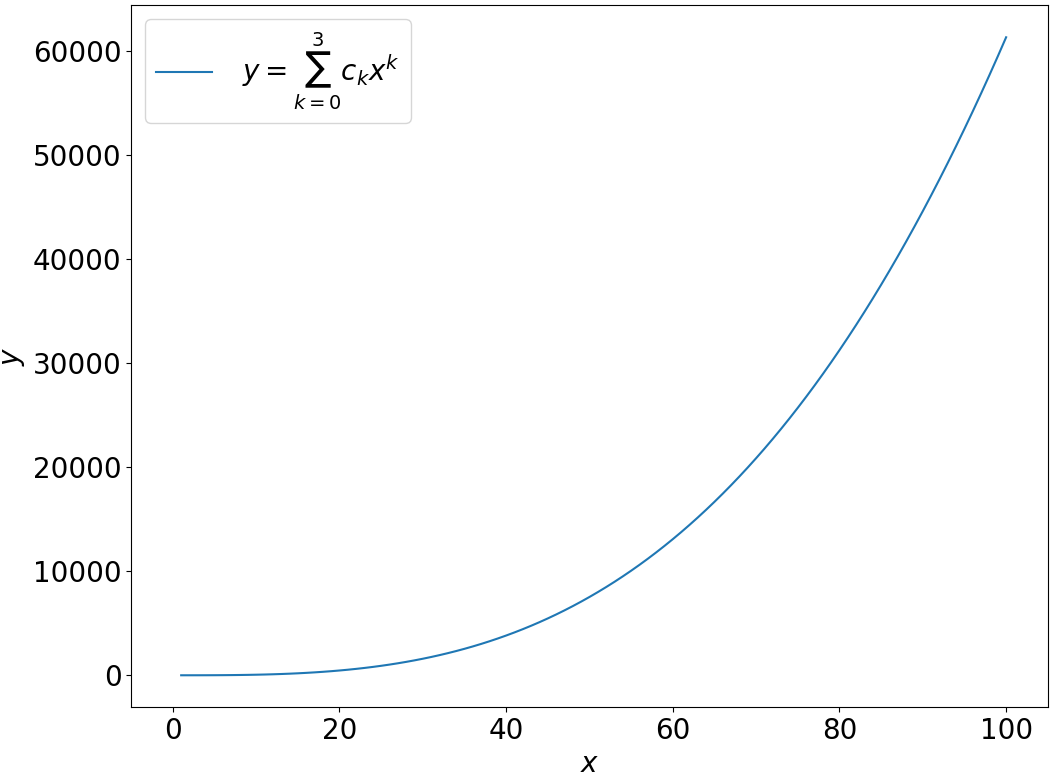
\includegraphics[width=\linewidth]{q3_N=3}
	\captionof{figure}{Plot of power series estimate of $f_{1}(x)$ for $N=3$}
	\label{q3_N=3}
\end{minipage}
\vspace{1cm}

\begin{minipage}{\textwidth}\centering
	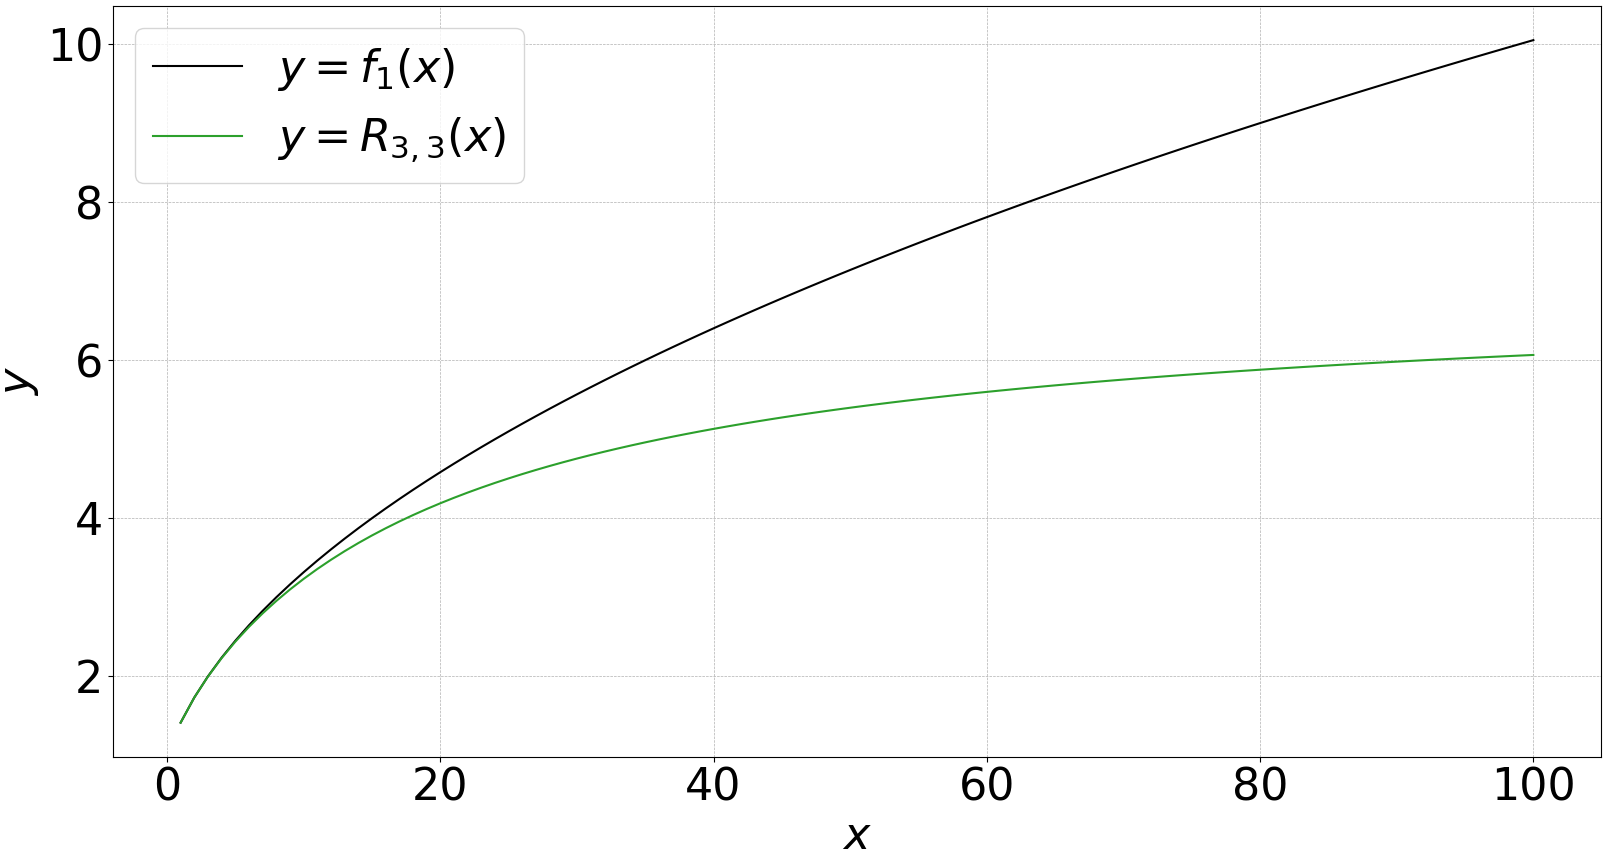
\includegraphics[width=0.8\linewidth]{q3_L=3}
	\label{q3_L=3}
\end{minipage}
\vspace{0.1cm}

\begin{minipage}{\textwidth}\centering
	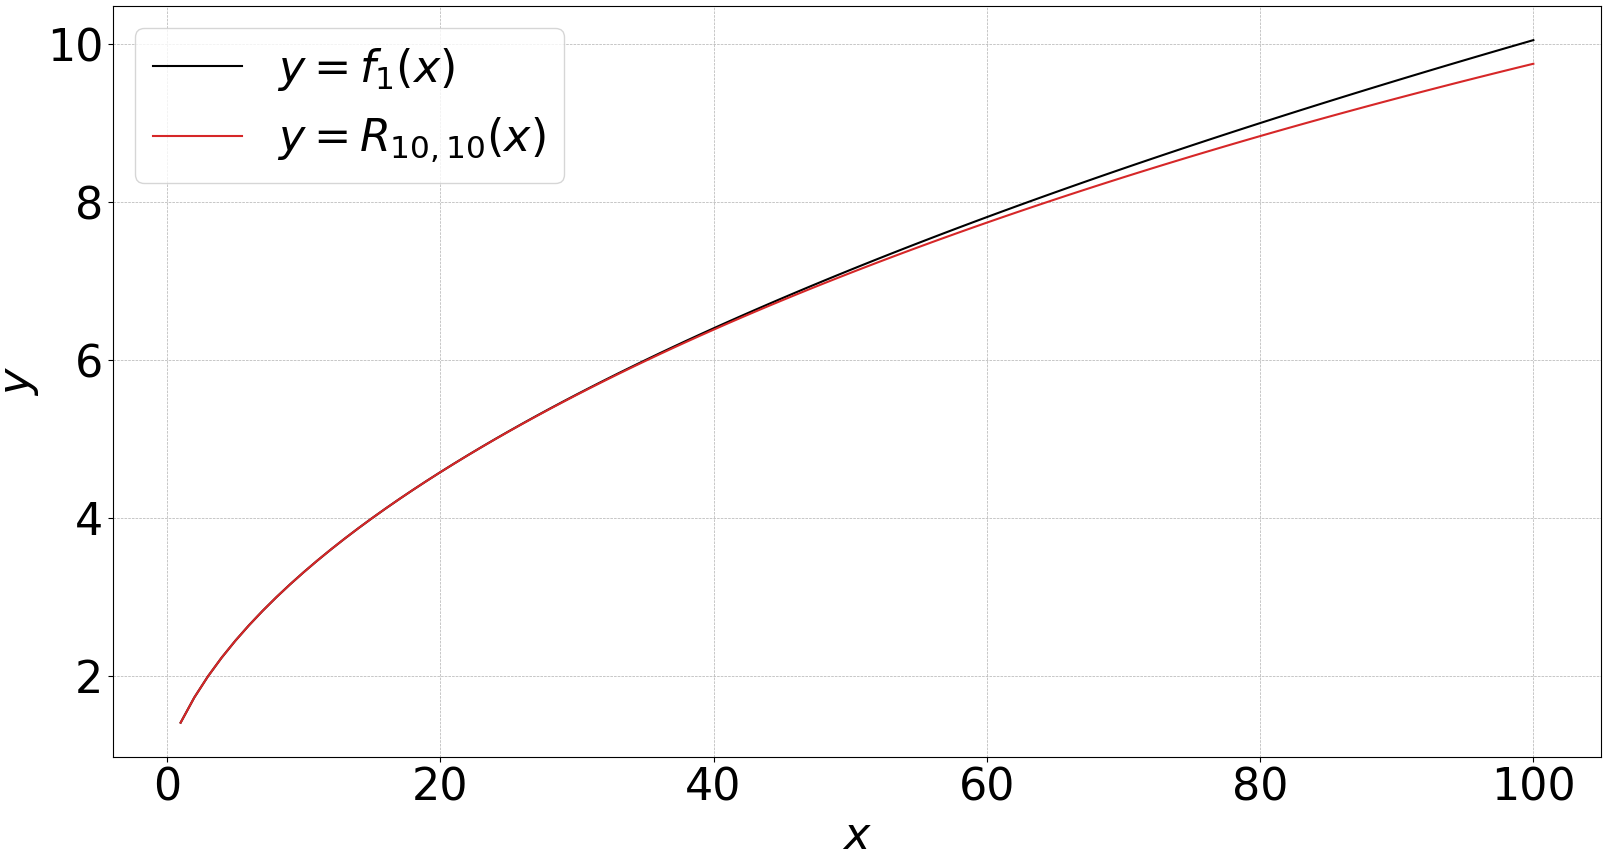
\includegraphics[width=0.8\linewidth]{q3_L=10}
	\label{q3_L=10}
\end{minipage}
\vspace{0.1cm}

\begin{minipage}{\textwidth}\centering
	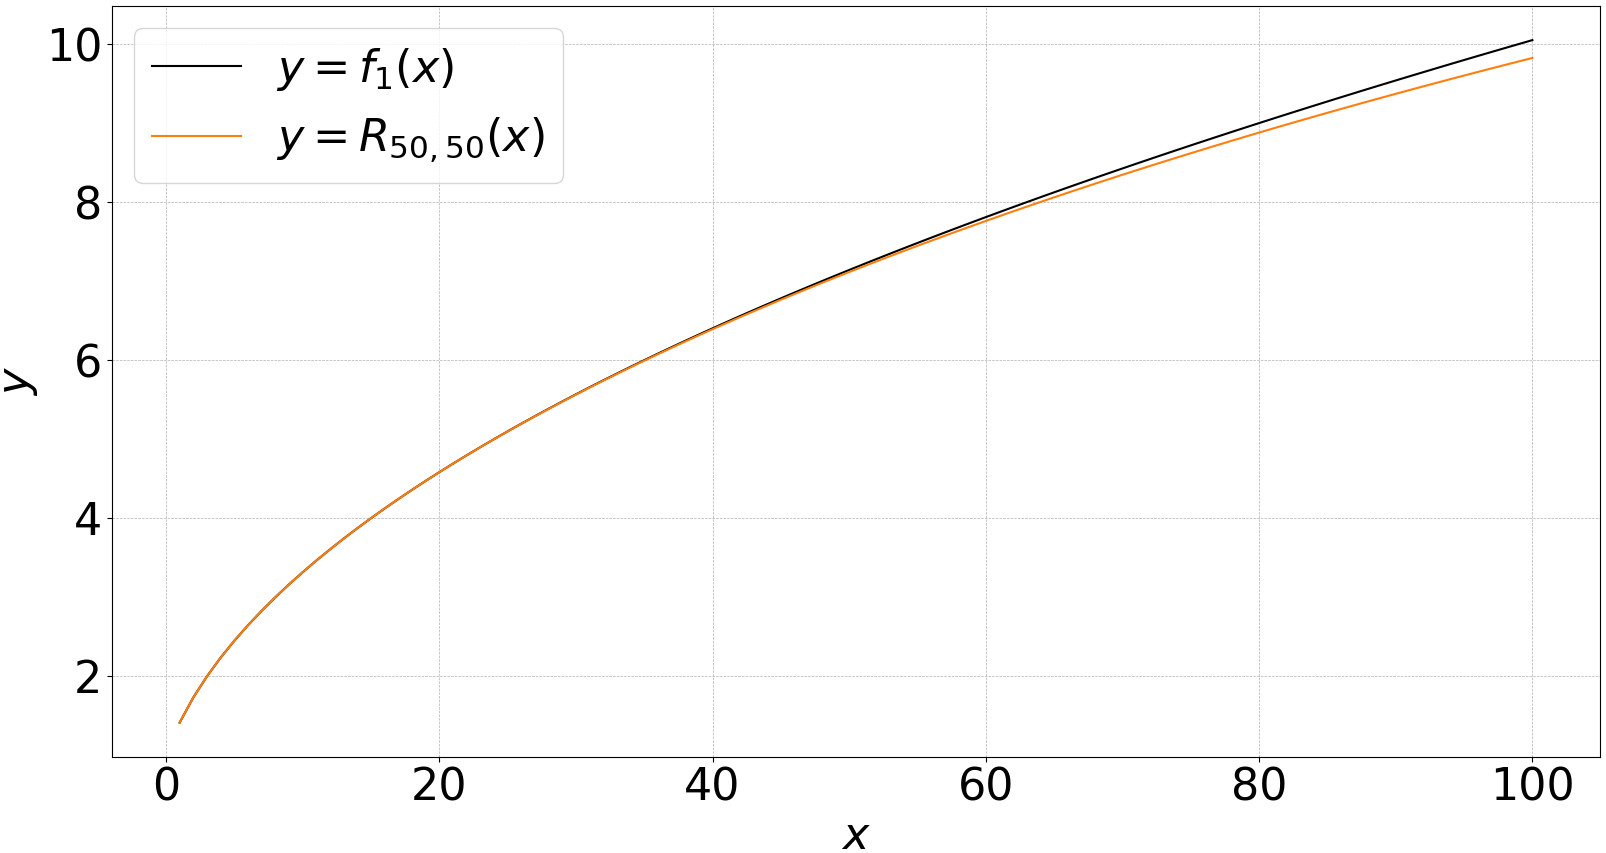
\includegraphics[width=0.8\linewidth]{q3_L=50}
	\captionof{figure}{Plots of Pad\'e approximant estimates of $f_{1}(x)$ for $L = 3, 10$ and $50$}
	\label{q3_L=50}
\end{minipage}
\vspace{0.1cm}

We can see from figure \ref{q3_N=3} that for $N=3$, the estimate increases at a rate of $x^{N}$.\ 
This means it diverges from $f_{1}(x)$ and for larger $N$ the estimate diverges even more quickly. This is\ 
because of the $x^{N}$ term in the power series which becomes very large for $x > 1$.
\\

In comparion, the diagonal Pad\'e approximant with $L=3$ stays much closer to $f_{1}(x)$ than the power series\ 
estimate. This is due to the fact that the Pad\'e approximant is a fraction so its limiting behaviour as\ 
$x \to \infty$ is much more similar to $f_{1}(x)$ than the power series' behaviour is. However, $L = 3$ does\ 
not give a good estimate in the range $1 \leq x \leq 100$. We see that for $L = 10$ and $L = 50$, we obtain\ 
much closer estimates while the power series would only diverge further.
\\

\begin{minipage}{\textwidth}\centering
	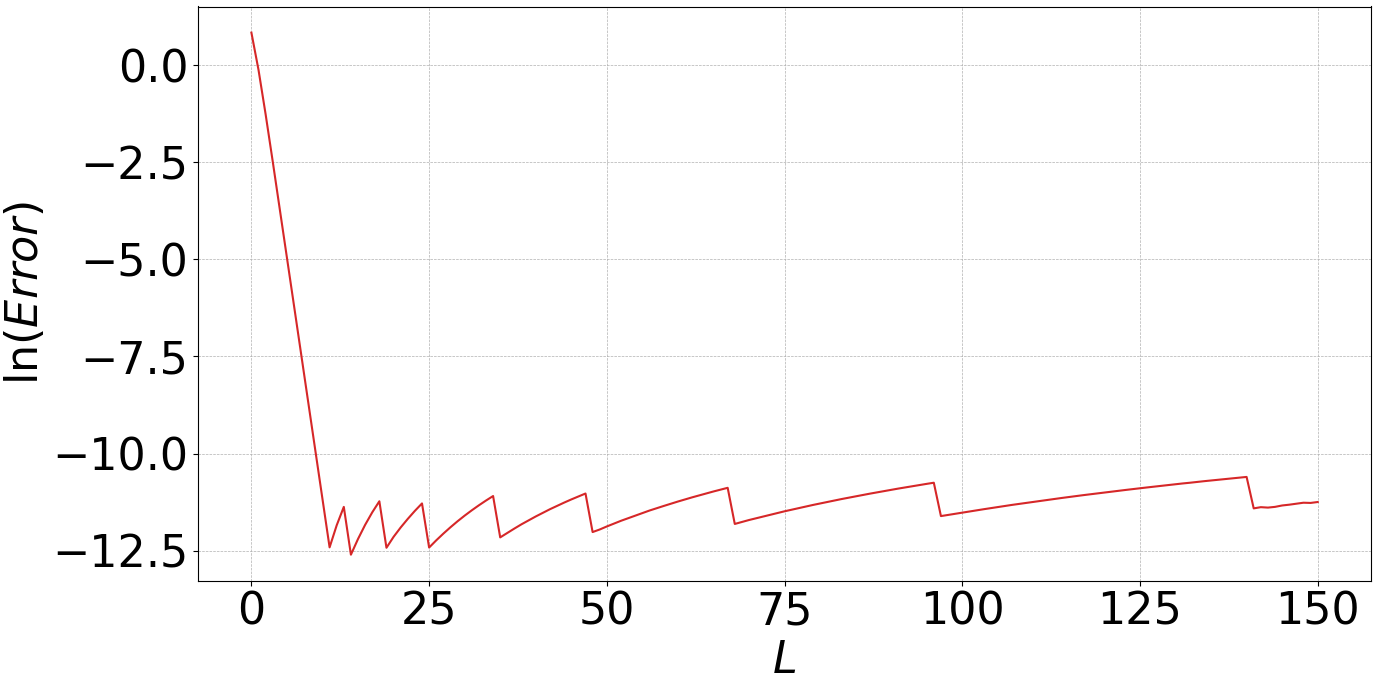
\includegraphics[width=\linewidth]{q3_fig3}
	\captionof{figure}{Plot $L$ against $\ln(error)$ for $x = 10$}
	\label{q3_fig3}
\end{minipage}
\vspace{1cm}

\begin{minipage}{\textwidth}\centering
	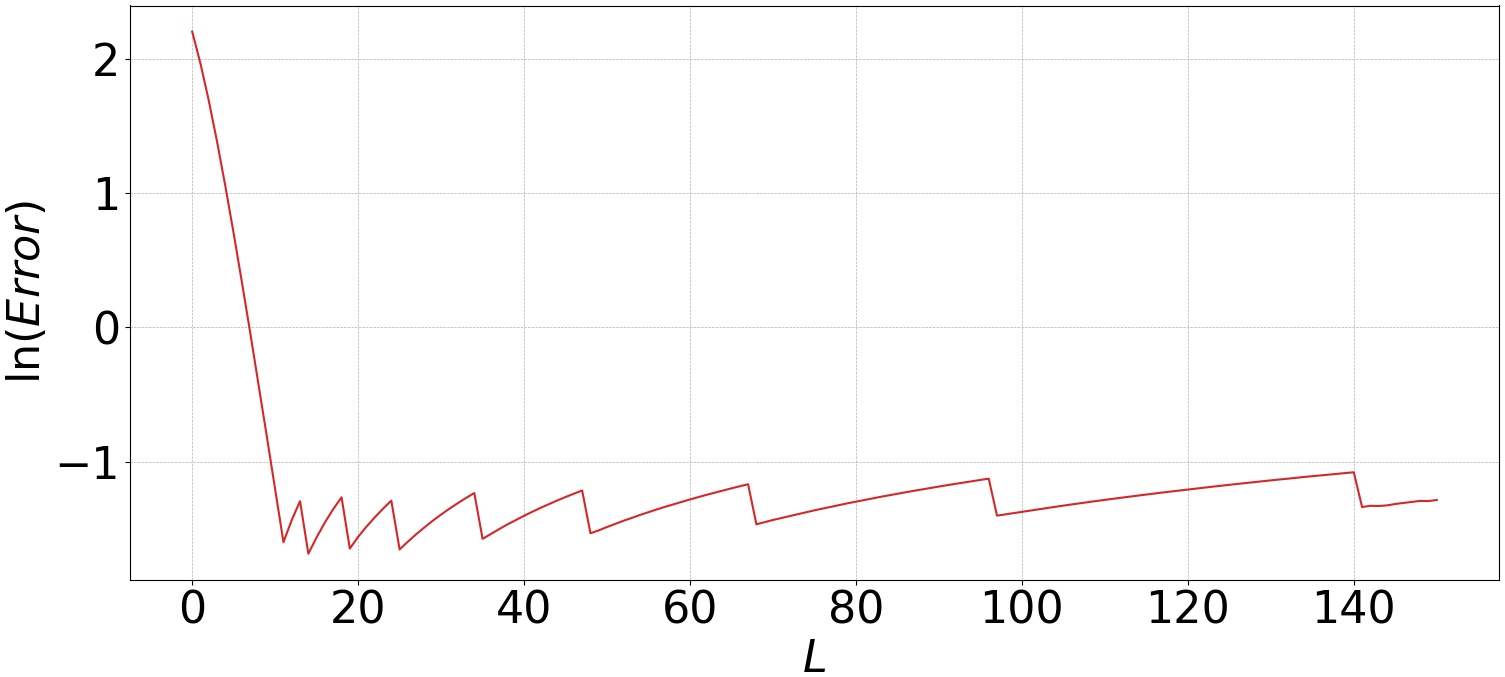
\includegraphics[width=\linewidth]{q3_fig4}
	\captionof{figure}{Plot $L$ against $\ln(error)$ for $x = 100$}
	\label{q3_fig4}
\end{minipage}
\vspace{1cm}

- Exponential decrease up to L = 10

- Same value of L as for x = 1. WHY?

- Apprears to be (can't be certain since haven't/can't test higher L) limit to minimum error. WHY?

- Around this minimimum value we get distinctive zig-zaggin. WHY ZIG-ZAGGING?
\\

Overall, we can see that the Pad\'e approximant almost converges to $f_{1}(x)$ for large $x$ despite\ 
the fact that this is outside the radius of convergence of the power series. However, there is a\ 
limitation on the accuracy of the estimate you can get where increasing the value of $L$ will not\ 
improve the result.
% ONE MORE IMPLICATION



\pagebreak
\textbf{Program\textunderscore A.py for Programming Task}\centering\label{Program_A}
\lstinputlisting[language=Python]{C:/Users/angus/OneDrive/Documents/CATAM 7.5/Program_A.py}
\vspace{2cm}

\pagebreak
\textbf{Program\textunderscore B.py for Programming Task}\centering\label{Program_B}
\lstinputlisting[language=Python]{C:/Users/angus/OneDrive/Documents/CATAM 7.5/Program_B.py}
\vspace{2cm}

\pagebreak
\textbf{Question\textunderscore 1.py for Question 1}\centering\label{Question_1}
\lstinputlisting[language=Python]{C:/Users/angus/OneDrive/Documents/CATAM 7.5/Question_1.py}
\vspace{2cm}


\end{document}